The integral described in Equation~\eqref{eq:signal} contains an $\epsilon_{vtx}$ parameter that describes the number of events we can reconstruct beyond the $zCut$ and includes both detector acceptance and inefficiencies. Using A' Monte Carlo, $\epsilon_{vtx}$ is calculated and the efficiency is parameterized as a function of mass and $z$ vertex position. At each mass, the ratio of the reconstructed to generated heavy photon events is scaled such that for L1L1, the fitted ratio is 1 at that target position. The reconstruction efficiency at the target without scaling is shown in Figure~\ref{fig:rawEff}.

\begin{figure}[H]
  \centering
      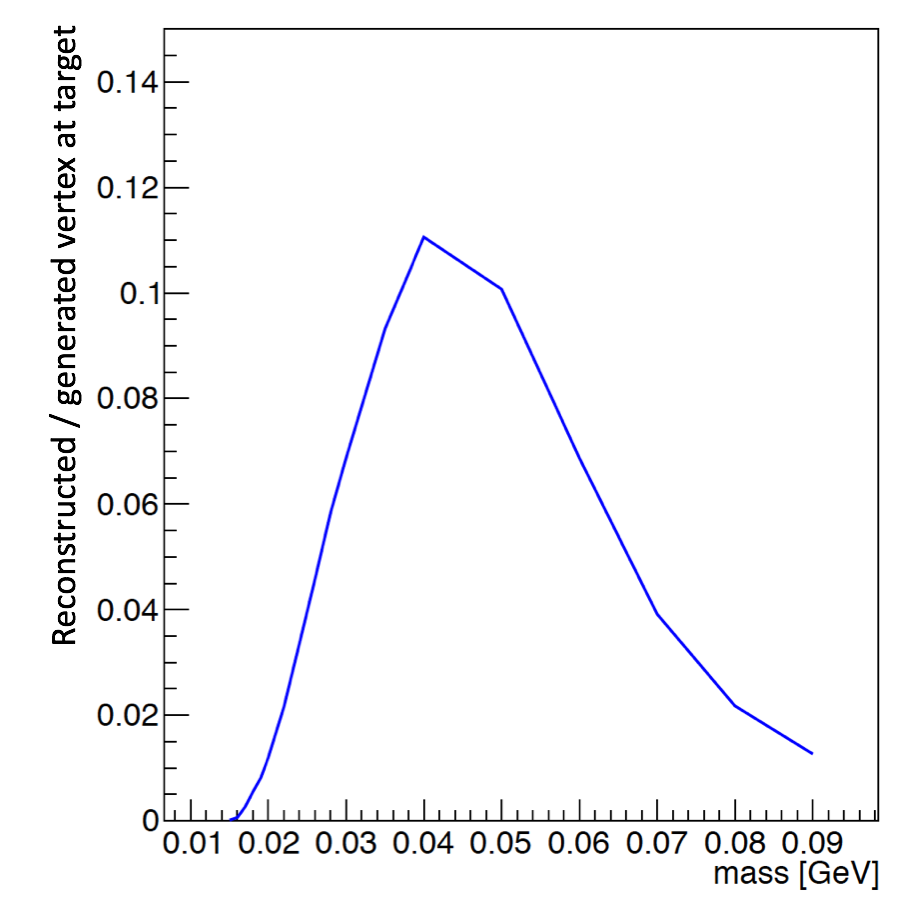
\includegraphics[width=0.8\textwidth]{pics/searching/rawEffL1L1.png}
  \caption[Reconstruction efficiency for heavy photons that decay at the target]{Reconstruction efficiency for heavy photon events with decay vertices at the target as a function of mass.}
  \label{fig:rawEff}
\end{figure} 

As shown in Figure~\ref{fig:rawEff}, the maximum efficiency in the HPS detector for events that decay promptly occurs around heavy photon masses between 40-50~MeV. This reconstruction efficiency at the target is normalized to 1, and the L1L2 and L2L2 data sets are scaled to ensure the same relative relationship between the three data sets. The reconstruction efficiencies for a 35~MeV heavy photon as a function of position are shown in Figure~\ref{fig:apEff}. 

\begin{figure}[H]
  \centering
      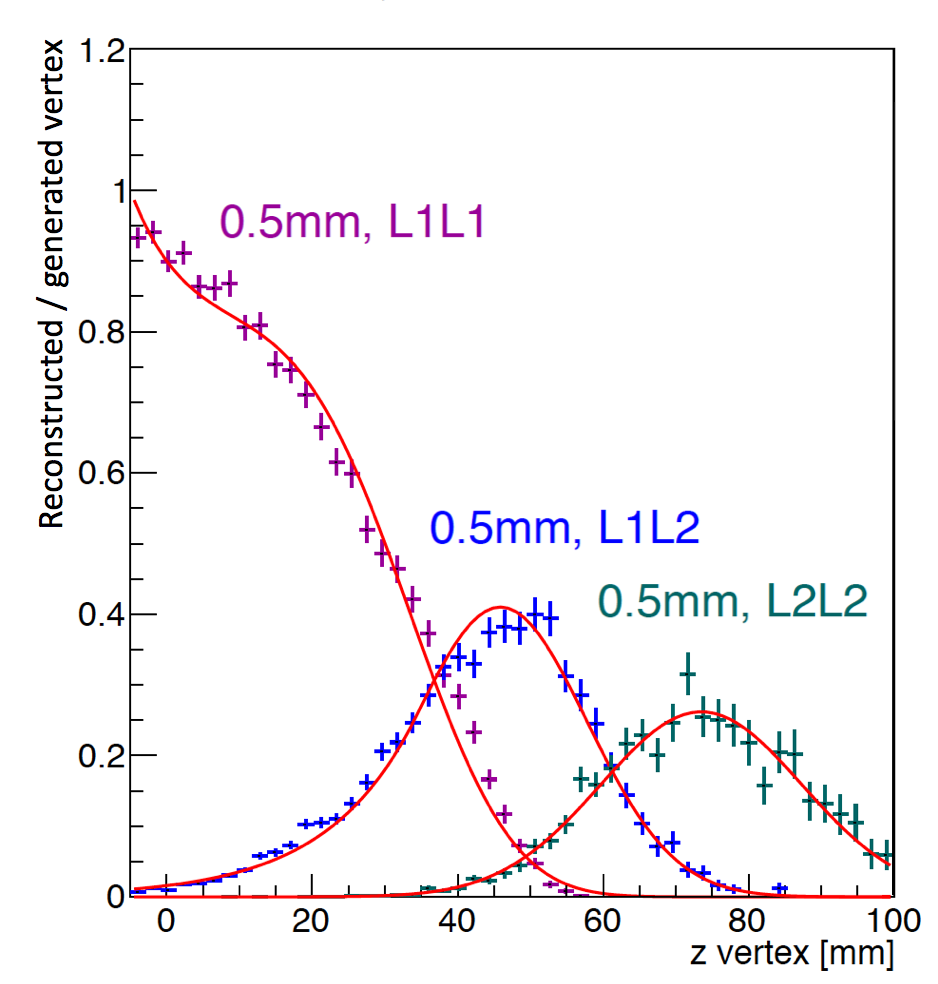
\includegraphics[width=0.8\textwidth]{pics/searching/reconstructedVtx.png}
  \caption[Fraction of reconstructed events of a 35~MeV A$^{\prime}$ as a function of decay vertex position]{Fraction of reconstructed events of a 35~MeV A$^{\prime}$ as a function of decay vertex position. The three datasets are mutually exclusive. Each data set is fit independently of the others and parameterized in terms of mass and $z$ vertex position. }
  \label{fig:apEff}
\end{figure} 

As shown in Figure~\ref{fig:apEff}, as all data sets are mutually exclusive of each other, the total reconstruction efficiency for all z vertex positions is the sum of the efficiencies for the individual datasets. These efficiencies are then integrated from different $zCut$ values to $zMax$ (roughly set at the z position of Layer 1, or 10~cm). The efficiency at each mass for each data set is fitted with a corresponding functional description that is parameterized in terms of mass and $z$ vertex position. The vertex reconstruction efficiency for the L1L1 data is described by Equation~\eqref{eq:promptfunction}.

\begin{equation}
\label{eq:promptfunction}
\epsilon_{vtx} = exp(p_0+p_1z+p_2z^2+p_3z^3) 
\end{equation}

In Equation~\eqref{eq:promptfunction}, all parameters are functions of mass. For the L1L2 data, the reconstruction efficiency turns on farther downstream and is described by a Crystal Ball function as shown in Equation~\eqref{eq:cbfunction}.

\begin{eqnarray*}
\label{eq:cbfunction}
\epsilon_{vtx}(t >= -| \alpha |) & = & N e^{-0.5t^{2}}\\
\epsilon_{vtx}(t < -| \alpha |) & = & N A(B-t)^{-n}\\
\textsf{where:}\\
\alpha & = & 0.97\\
n & = & 141.5\\
t & = & \dfrac{z-z_{mean}}{\sigma}\\
A & = & (\dfrac{n}{| \alpha |})^{n}e^{-0.5 |\alpha |^2}\\
B & = & \dfrac{n}{| \alpha |}-|\alpha | \\
N & = & \textsf{amplitude of the Gaussian}
\end{eqnarray*}

From Equation~\eqref{eq:cbfunction}, the parameters $z_{mean}$, $\sigma$, and $N$ are obtained from fitting the distribution and are functions of mass. The L2L2 data set efficiency turns on farther downstream than L1L2 and is best described by a Gaussian as in Equation~\eqref{eq:gausfunction}.

\begin{equation}
\label{eq:gausfunction}
Ne^{-0.5\dfrac{(z-z_{mean})^2}{\sigma^2}}
\end{equation}

The individual fit parameter values are described numerically in ~\ref{appendix:vtxEff}.\\
\indent Once these relations are derived, we obtain a value for $\epsilon_{vtx}$ that is integrated from the $zCut$ to the maximum $zMax$ when calculating the expected signal yield. The full integral is shown in Figure~\ref{fig:effIntegral} as the color z-axis and is a function of both the heavy photon mass and $zCut$.  

\begin{figure}[H]
  \centering
      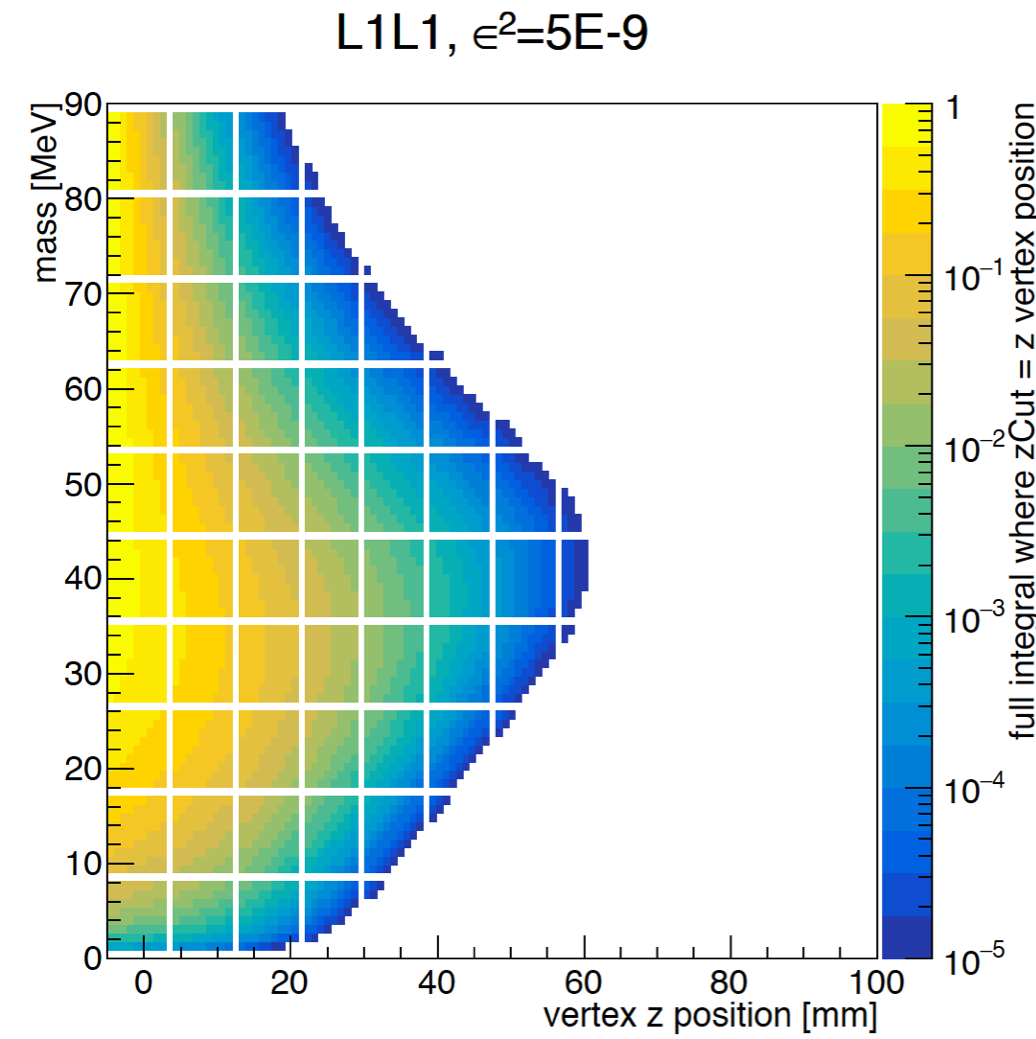
\includegraphics[width=0.8\textwidth]{pics/searching/integralEffL1L1.png}
  \caption[Integral as a function of mass and $zCut$ for L1L1]{The z-axis shows the color corresponding to the integral value for the L1L1 0.5~mm data set as a function of the $zCut$ and mass. The coupling, $\epsilon^2$ is fixed here to $5E-9$ and $zMax$ is chosen to be 10~cm, corresponding to the $z$ position of the first SVT layer. }
  \label{fig:effIntegral}
\end{figure}

The full integral value yields some fractional number that, when multiplied by the expected heavy photon yield from the cross section, tells us how many heavy photons we can expect to reconstruct in the given decay vertex region. For the L1L1 dataset, it is critical to set the zCut as low as possible in order to obtain the highest signal yield. In Figure~\ref{fig:effIntegral}, the value of the integral indicated by the color on the z-axis, is shown for $\epsilon^{2} = 5E-9$ as a function of mass and $zCut$. The $zMax$ was set to 10~cm in this calculation. The same calculation is done for the L1L2 dataset at shown in Figure~\ref{fig:effIntegral12}.

\begin{figure}[H]
  \centering
      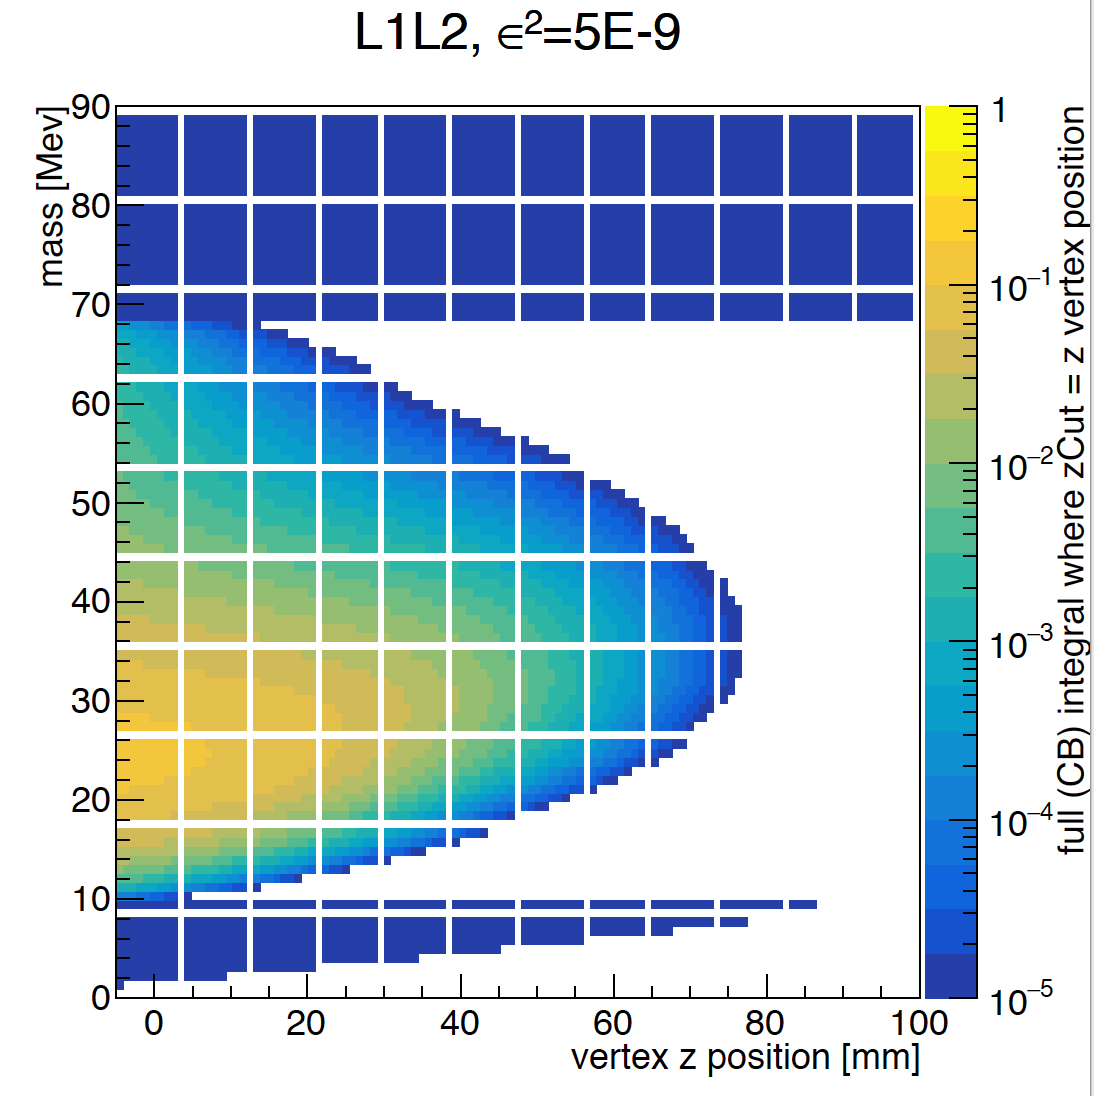
\includegraphics[width=0.8\textwidth]{pics/searching/integralEff12.png}
  \caption[Integral as a function of mass and $zCut$ for L1L2]{The z-axis shows the color corresponding to the integral value for the L1L2 0.5~mm data set as a function of the $zCut$ and mass. The coupling, $\epsilon^2$ is fixed here to $5E-9$ and $zMax$ is chosen to be 10~cm, corresponding to the $z$ position of the first SVT layer. }
  \label{fig:effIntegral12}
\end{figure}

In Figure~\ref{fig:effIntegral12}, the maximum fractional signal yield is significantly less than in the L1L1 data set. The lifetime of the heavy photon in Figure~\ref{fig:effIntegral12} is not long enough to significantly benefit from the additional efficiency obtained at longer displaced $z$ vertex positions. The integrated efficiency for the L2L2 data is shown in Figure~\ref{fig:effIntegral22}.

\begin{figure}[H]
  \centering
      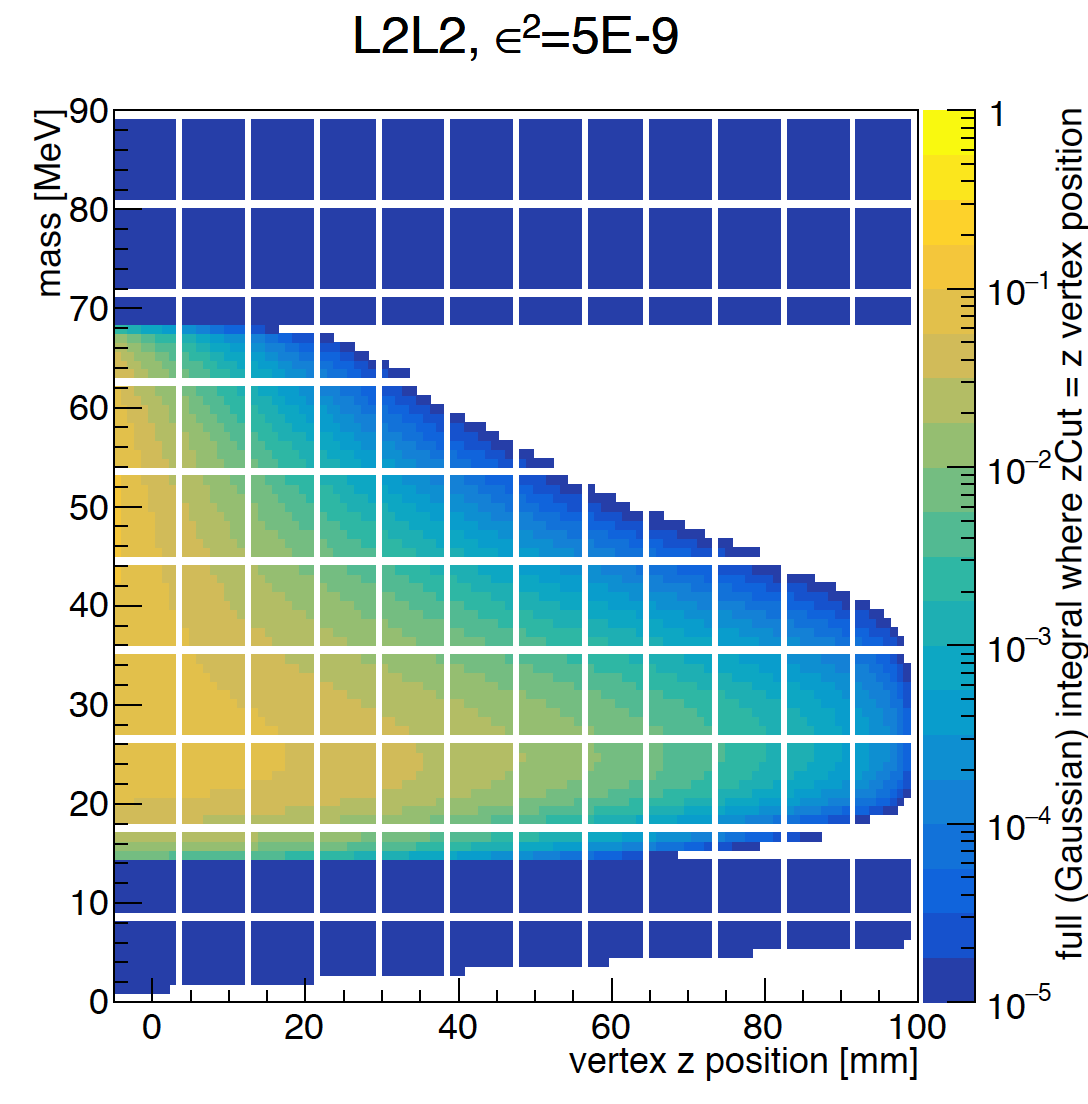
\includegraphics[width=0.8\textwidth]{pics/searching/integralEff22.png}
  \caption[Integral as a function of mass and $zCut$ for L2L2]{The z-axis shows the color corresponding to the integral value for the L2L2 0.5~mm data set as a function of the $zCut$ and mass. The coupling, $\epsilon^2$ is fixed here to $5E-9$ and $zMax$ is chosen to be 10~cm, corresponding to the $z$ position of the first SVT layer. }
  \label{fig:effIntegral22}
\end{figure}

As shown in Figure~\ref{fig:effIntegral22}, the fraction yield is significantly less when compared to the L1L1 dataset and requires a very small $zCut$ value in order to recover the maximum yield. Additionally, the L1L2 and L2L2 datasets are most beneficial for detecting lower mass A$^\prime$s with displaced $z$ vertex positions. 